\chapter{Experiment Setup}\label{ch:exp-setup}
This appendix provides supplementary tables and figures for the experimental setup described in Section \ref{sec:experiment_setup}. Section \ref{sec:exp-reward-setup} documents the exact reward configuration used by the greedy agent and during \ac{ppo} training. Section \ref{sec:exp-scenario-setup} shows the two evaluated power grids with their modified components highlighted, together with a full listing of all chosen scenarios and evaluation indices. Finally, Section \ref{sec:exp-ppo-setup} lists the tunable hyperparameters of the \ac{gnn}-based \ac{ppo} agent, the final tuned values for each scenario, and the results of the corresponding training runs.

\section{Reward Setup}\label{sec:exp-reward-setup}
Table \ref{tab:reward_settings} lists the metrics and their assigned weights used to compute the reward signal for the greedy agent's action selection and for training the \ac{ppo} agent, as introduced in Section \ref{sec:agent-integration}. The corresponding worst-case and best-case reference values used to normalise each metric are fixed and listed in Table \ref{tab:reward_metrics}.

\begin{table}[htbp]
  \centering
  \small
  \caption{Reward configuration used in all experiments}
  \label{tab:reward_settings}
  \begin{tabular}{lc}
    \toprule
    Metric & Weight $w_i$  \\
    \midrule
    Maximum line loading $N\!-\!0$ & 3 \\
    Number of overloaded lines $N\!-\!0$ & 1 \\
    \midrule
    Non-convergence penalty $r_{\mathrm{fail}}$ & $-2$ \\
    \bottomrule
  \end{tabular}
\end{table}

\FloatBarrier










\section{Scenario Setup}\label{sec:exp-scenario-setup}
This section documents the two power grids and all scenarios evaluated in the experiments, complementing the description given in Section \ref{sec:experiment_setup}.

\subsection{Evaluated Power Grids}
Figure \ref{fig:exp-grids} shows the two IEEE test grids used throughout the experiments, with the components affected by scenario-specific modifications, such as scaled generators or loads, highlighted directly on the grid layout.

\begin{figure}[htp]
    \centering
    \begin{subfigure}[b]{0.8\textwidth}
        \centering
        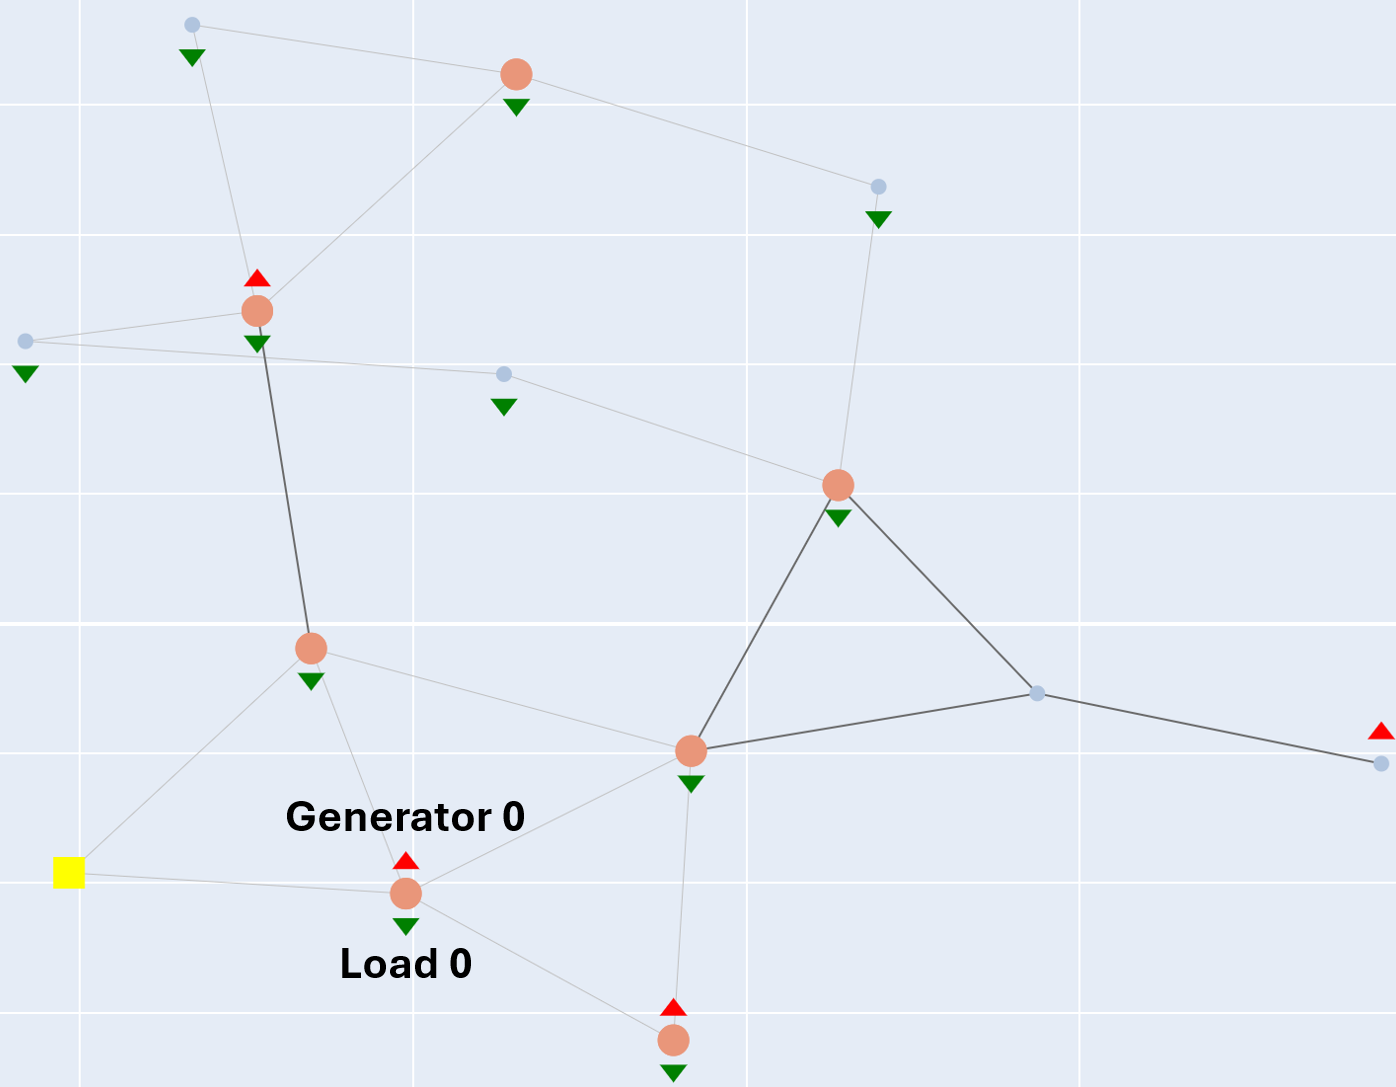
\includegraphics[width=\textwidth]{images/experiments/grids/14b.png}
        \caption{IEEE 14-bus test grid}
        \label{fig:grid-14}
    \end{subfigure}

    \vspace{1em}

    \begin{subfigure}[b]{1\textwidth}
        \centering
        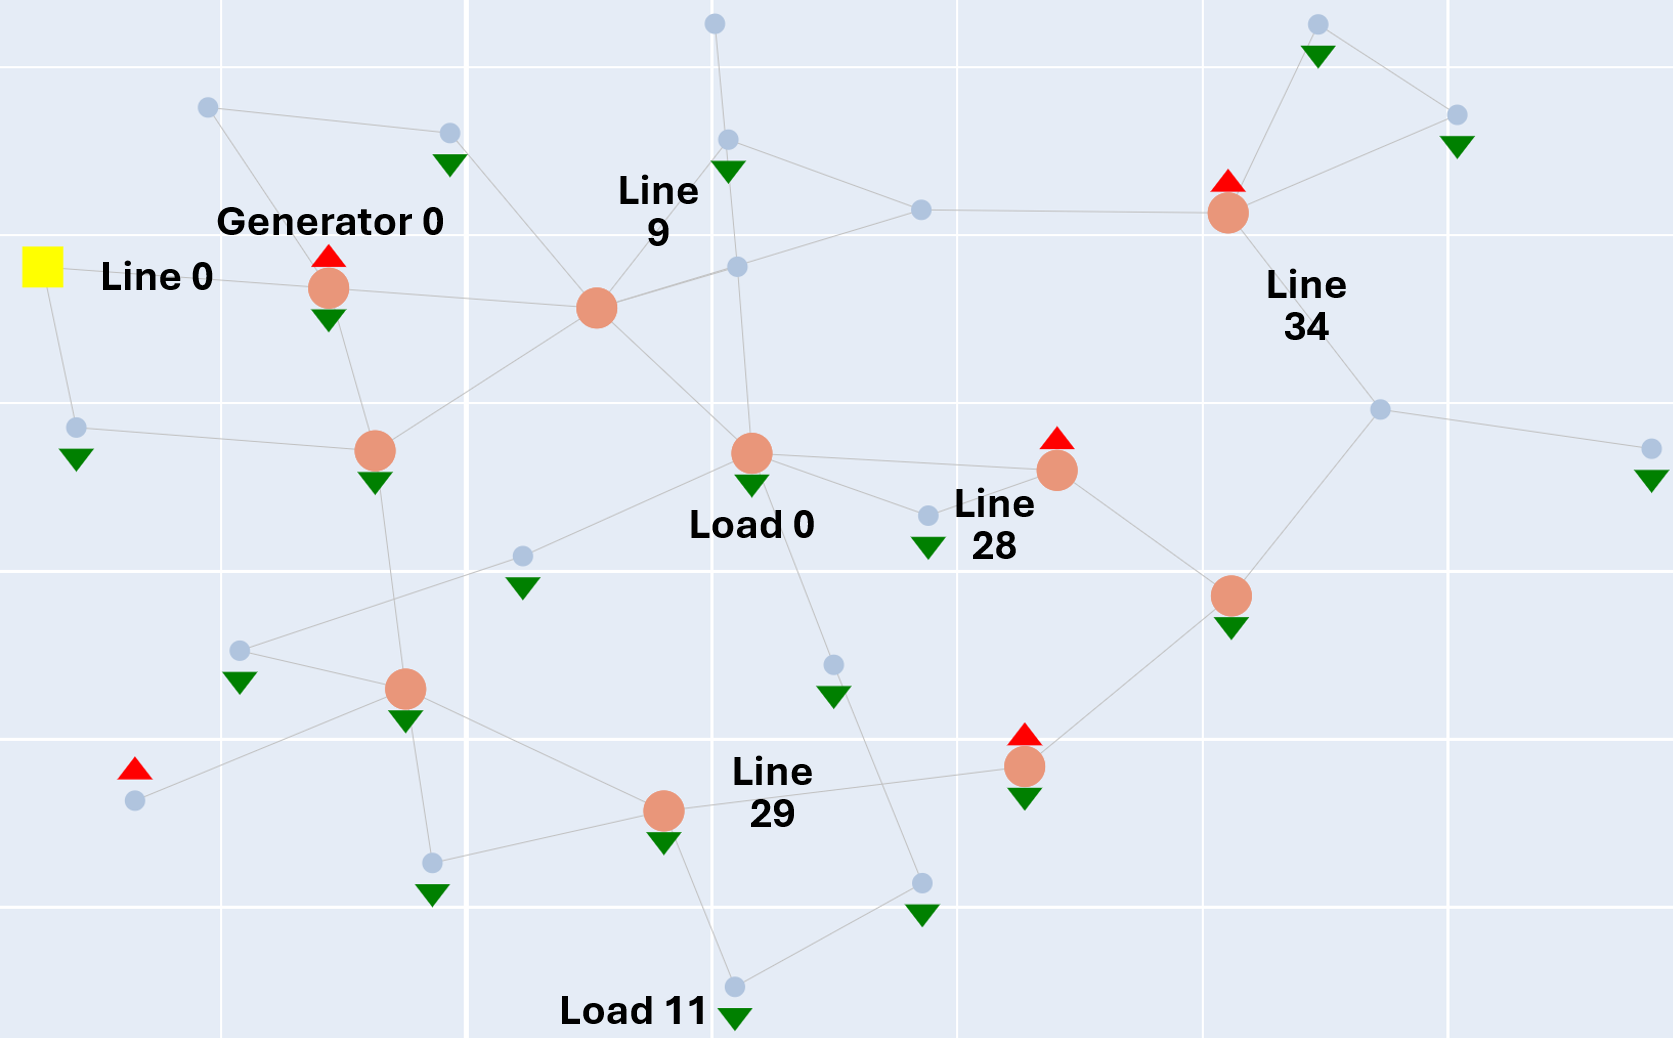
\includegraphics[width=\textwidth]{images/experiments/grids/30b.png}
        \caption{IEEE 30-bus test grid}
        \label{fig:grid-30}
    \end{subfigure}
    \caption{Power grids used in the experiments, with modified grid components identified by labels}
    \label{fig:exp-grids}
\end{figure}

\FloatBarrier

\subsection{Chosen Scenarios and Runs}
Table \ref{tab:scenarios-setup} lists all scenarios evaluated in the experiments, together with the profile day indices selected for each run and a short description of the modifications applied to the respective base grid, as introduced in Section \ref{sec:experiment_setup}.

\begin{table}[htbp]
\centering
\small
\renewcommand{\arraystretch}{1.3}
\begin{tabular}{|l|p{4.6cm}|p{6cm}|}
\hline
\textbf{Scenario Name} & \textbf{Index} & \textbf{Description} \\
\hline
14B\_ORIG & 1920, 8640, 21120 (days 20, 90, 220) & Unmodified 14-bus IEEE test case \\
\hline
14B\_UP\_GN0 & 3840, 18240, 26880 (days 40, 190, 280) & 14-bus case, active power generation of generator 0 scaled by $5\times$ (original 420\,MW) \\
\hline
14B\_UP\_LD0 & 3840, 11520, 5760 (days 40, 120, 60) & 14-bus case, active and reactive power of load 0 scaled by $15\times$ (original 65-70\,MW)\\
\hline
14B\_UP\_GN0- & 3840, 18240, 26880 (days 40, 190, 280) & As 14B\_UP\_GN0, but with a lower scaling factor of $2.5\times$ \\
\hline
14B\_UP\_GN0+ & 3840, 18240, 26880 (days 40, 190, 280) & As 14B\_UP\_GN0, but with a higher scaling factor of $7.5\times$ \\
\hline
14B\_UP\_LD0- & 3840, 11520, 5760 (days 40, 120, 60) & As 14B\_UP\_LD0, but with a lower scaling factor of $5\times$ \\
\hline
14B\_UP\_LD0+ & 3840, 11520, 5760 (days 40, 120, 60) & As 14B\_UP\_LD0, but with a higher scaling factor of $25\times$ \\
\hline
30B\_ORIG & 27840 (day 290) & Unmodified 30-bus IEEE test case \\
\hline
30B\_UP\_LD5 & 12480, 13440, 30720 (days 130, 140, 320) & 30-bus case, active and reactive power of load 5 scaled by $20\times$ (original 3\,MW) \\
\hline
30B\_UP\_LD11 & 10560, 13440, 27840 (days 110, 140, 290) & 30-bus case, active and reactive power of load 11 scaled by $20\times$ (original 3\,MW) \\
\hline
30B\_MT\_LN & 27840 (day 290) & 30-bus case, year-long maintenance outage of lines 0, 9, 28, 29 and 34 \\
\hline
30B\_MT\_GN & 27840 (day 290) & 30-bus case, year-long maintenance outage of generator 0 \\
\hline
30B\_RC\_LN & 27840 (day 290) & 30-bus case, thermal capacity of lines 0, 9, 28, 29 and 34 reduced to 25\,\% \\
\hline
30B\_RC\_LN- & 27840 (day 290) & As 30B\_RC\_LN, but with a milder reduction to 50\,\% \\
\hline
30B\_RC\_LN+ & 27840 (day 290) & As 30B\_RC\_LN, but with a stronger reduction to 10\,\% \\
\hline
\end{tabular}
\caption{Overview of the scenarios and their evaluation indices for each run}
\label{tab:scenarios-setup}
\end{table}

\FloatBarrier












\section{PPO Setup}\label{sec:exp-ppo-setup}
This section documents the hyperparameters of the \ac{gnn}-based \ac{ppo} agent introduced in Section \ref{ssec:custom-agent-setup}, the final values selected for each scenario by the \texttt{OptunaTuner}, and the outcome of the corresponding training runs.

\subsection{Hyperparameters}
Table \ref{tab:ppo-hparams} lists and briefly describes all tunable hyperparameters of the \ac{gnn}-based \ac{ppo} agent, grouped by the component of the architecture they belong to. Then, Table \ref{tab:hparams-ieee14} and \ref{tab:hparams-ieee30} report the final tuned hyperparameter values selected for the seven 14-bus scenarios and eight 30-bus scenarios.

\newcommand{\hprule}{\cmidrule(l){2-3}}
\begin{table}[htbp]
  \centering
  \footnotesize 
  \caption{Hyperparameters of the \ac{gnn}-based \ac{ppo} agent}
  \label{tab:ppo-hparams}
  \begin{tabularx}{\textwidth}{@{}llX@{}}
    \toprule
    \textbf{Component} & \textbf{Hyperparameter} & \textbf{Description} \\
    \midrule
    \multirow{6}{*}{GINE encoder}
        & \texttt{gine\_hidden\_dims}     & GINEConv hidden dimensions; list length defines the number of layers and each value the layer width. \\
        \hprule
        & \texttt{gine\_mlp\_layers}      & Number of layers of the \ac{mlp} inside each GINEConv operator \\
        \hprule
        & \texttt{gine\_mlp\_activation}  & Activation function of these \acp{mlp} \\
        \hprule
        & \texttt{pooling}                & Readout operator that aggregates the node embeddings into a single graph embedding: \texttt{mean} (average over all buses), \texttt{add} (sum over all buses) or \texttt{max} (element-wise maximum over all buses). \\
        \hprule
        & \texttt{norm}                   & Normalisation scheme applied between the graph convolutions: \texttt{layer} (layer normalisation per node embedding), \texttt{graph} (normalisation across all nodes of a graph) or \texttt{none}. \\
        \hprule
        & \texttt{dropout}                & Dropout probability in the encoder, randomly deactivates a fraction of the values in bus embeddings during training steps, forcing the network to distribute information across many features to reduce overfitting \\
    \midrule
    \multirow{2}{*}{Policy head}
        & \texttt{fc\_hidden\_dims}       & Width and depth of the fully connected layers that output the action logits and the value estimate \\
        \hprule
        & \texttt{fc\_activation}         & Activation function of the fully connected head \\
    \midrule
    \multirow{9}{*}{\ac{ppo}}
        & \texttt{train\_batch\_size}     & Number of environment steps collected per training iteration \\
        \hprule
        & \texttt{minibatch\_size}        & Size of the \ac{sgd} minibatches into which the training batch is split \\
        \hprule
        & \texttt{num\_epochs}            & Number of passes over the collected batch per training iteration \\
        \hprule
        & \texttt{lr}                     & Learning rate of the optimiser \\
        \hprule
        & \texttt{gamma}                  & Discount factor $\gamma$ weighting future rewards \\
        \hprule
        & \texttt{lambda\_}               & \ac{gae} parameter $\lambda$, trading bias against variance in the advantage estimate \\
        \hprule
        & \texttt{entropy\_coeff}         & Weight of the entropy bonus, controlling exploration of the discrete action space \\
        \hprule
        & \texttt{clip\_param}            & Clipping range of the policy ratio, limiting the size of a policy update \\
        \hprule
        & \texttt{vf\_clip\_param}        & Clipping range of the value-function loss \\
    \midrule
    Rollouts
        & \texttt{num\_envs\_per\_env\_runner} & Number of vectorised environments per rollout worker \\
    \bottomrule
  \end{tabularx}
\end{table}

\begin{table}[htbp]
  \centering
  \small
  \caption{Final tuned hyperparameter values for the seven IEEE case~14 scenarios}
  \label{tab:hparams-ieee14}
  \resizebox{\textwidth}{!}{%
  \begin{tabular}{@{}llrrrrrrr@{}}
    \toprule
    \textbf{Component} & \textbf{Hyperparameter} & \textbf{ORI} & \textbf{G0} & \textbf{G0-H} & \textbf{G0-L} & \textbf{L0} & \textbf{L0-H} & \textbf{L0-L} \\
    \midrule
    \multirow{6}{*}{GINE encoder}
      & \texttt{gine\_hidden\_dims}    & [4$\times$256] & [4$\times$128] & [5$\times$256] & [2$\times$128] & [3$\times$128] & [2$\times$256] & [4$\times$128] \\
      & \texttt{gine\_mlp\_layers}     & 3 & 3 & 4 & 3 & 3 & 3 & 3 \\
      & \texttt{gine\_mlp\_activation} & relu & relu & relu & relu & relu & elu & elu \\
      & \texttt{pooling}               & mean & mean & mean & mean & mean & mean & mean \\
      & \texttt{norm}                  & layer & layer & none & layer & layer & layer & layer \\
      & \texttt{dropout}               & 0.0249 & 0.0446 & 0.0720 & 0.0477 & 0.0582 & 0.1031 & 0.0329 \\
    \midrule
    \multirow{2}{*}{Policy head}
      & \texttt{fc\_hidden\_dims}      & [256] & [256] & [256,\,256] & [256,\,256] & [512] & [256] & [256] \\
      & \texttt{fc\_activation}        & elu & elu & elu & elu & elu & elu & elu \\
    \midrule
    \multirow{9}{*}{PPO}
      & \texttt{train\_batch\_size}    & 2048 & 2048 & 2048 & 2048 & 2048 & 2048 & 2048 \\
      & \texttt{minibatch\_size}       & 512 & 2048 & 2048 & 512 & 2048 & 2048 & 512 \\
      & \texttt{num\_epochs}           & 1 & 1 & 7 & 1 & 2 & 7 & 1 \\
      & \texttt{lr}                    & 2.32e-5 & 1.81e-4 & 3.27e-5 & 1.68e-5 & 1.02e-4 & 3.33e-5 & 3.86e-5 \\
      & \texttt{gamma}                 & 0.9769 & 0.9748 & 0.9588 & 0.9786 & 0.9749 & 0.9587 & 0.9884 \\
      & \texttt{lambda\_}              & 0.9314 & 0.9248 & 0.9748 & 0.9182 & 0.9065 & 0.9391 & 0.9622 \\
      & \texttt{entropy\_coeff}        & 1.09e-3 & 1.00e-3 & 7.98e-3 & 1.04e-2 & 1.20e-3 & 1.00e-3 & 1.02e-3 \\
      & \texttt{clip\_param}           & 0.3181 & 0.3421 & 0.3946 & 0.3643 & 0.2823 & 0.3457 & 0.3098 \\
      & \texttt{vf\_clip\_param}       & 27.01 & 23.05 & 33.82 & 20.11 & 12.67 & 13.54 & 30.52 \\
    \midrule
    Rollouts
      & \texttt{num\_envs\_per\_env\_runner} & 8 & 8 & 4 & 16 & 8 & 8 & 16 \\
    \bottomrule
  \end{tabular}}

  \vspace{0.5em}
  \begin{minipage}{\textwidth}
    \footnotesize
    \textbf{Legend:}
    \textbf{ORI}: \texttt{original} (unmodified grid);
    \textbf{G0}: \texttt{upscale\_gen0\_downscale\_rest};
    \textbf{G0-H} / \textbf{G0-L}: high / low variant of the same scenario;
    \textbf{L0}: \texttt{upscale\_load0\_downscale\_rest};
    \textbf{L0-H} / \textbf{L0-L}: high / low variant thereof.
    \emph{high} and \emph{low} refer to the magnitude of the up-/downscaling factor applied to the
    generator or load at the indicated bus. Entries such as
    \mbox{[4$\times$256]} denote a list of four GINEConv layers of width 256;
    \mbox{[256]} denotes a single fully connected layer of width 256 and
    \mbox{[256,\,256]} two fully connected layers of width 256 each.
  \end{minipage}
\end{table}

\begin{table}[htbp]
  \centering
  \small
  \caption{Final tuned hyperparameter values for the eight IEEE case~30 scenarios}
  \label{tab:hparams-ieee30}
  \resizebox{\textwidth}{!}{%
  \begin{tabular}{@{}llrrrrrrrr@{}}
    \toprule
    \textbf{Component} & \textbf{Hyperparameter} & \textbf{ORI} & \textbf{RLC} & \textbf{RLC-H} & \textbf{RLC-L} & \textbf{MG} & \textbf{ML} & \textbf{L5} & \textbf{L11} \\
    \midrule
    \multirow{6}{*}{GINE encoder}
      & \texttt{gine\_hidden\_dims}    & [3$\times$128] & [4$\times$256] & [4$\times$256] & [3$\times$256] & [4$\times$256] & [3$\times$512] & [4$\times$256] & [5$\times$512] \\
      & \texttt{gine\_mlp\_layers}     & 3 & 2 & 2 & 2 & 2 & 2 & 3 & 4 \\
      & \texttt{gine\_mlp\_activation} & relu & elu & elu & elu & elu & elu & relu & relu \\
      & \texttt{pooling}               & mean & add & add & add & add & mean & mean & mean \\
      & \texttt{norm}                  & layer & none & graph & none & graph & none & graph & none \\
      & \texttt{dropout}               & 0.0582 & 0.0348 & 0.1985 & 0.1072 & 0.0087 & 0.0459 & 0.0166 & 0.1147 \\
    \midrule
    \multirow{2}{*}{Policy head}
      & \texttt{fc\_hidden\_dims}      & [512] & [256] & [256] & [256] & [256,\,256] & [256] & [512] & [128,\,128] \\
      & \texttt{fc\_activation}        & elu & relu & relu & elu & relu & elu & relu & elu \\
    \midrule
    \multirow{9}{*}{PPO}
      & \texttt{train\_batch\_size}    & 2048 & 4096 & 4096 & 4096 & 4096 & 4096 & 4096 & 4096 \\
      & \texttt{minibatch\_size}       & 2048 & 2048 & 1024 & 2048 & 1024 & 1024 & 1024 & 2048 \\
      & \texttt{num\_epochs}           & 2 & 7 & 7 & 7 & 4 & 4 & 4 & 1 \\
      & \texttt{lr}                    & 1.02e-4 & 6.18e-5 & 3.14e-5 & 7.41e-5 & 2.27e-5 & 2.03e-5 & 3.08e-5 & 8.38e-5 \\
      & \texttt{gamma}                 & 0.9749 & 0.9594 & 0.9532 & 0.9508 & 0.9593 & 0.9581 & 0.9727 & 0.9749 \\
      & \texttt{lambda\_}              & 0.9065 & 0.9452 & 0.9318 & 0.9691 & 0.9288 & 0.9440 & 0.9017 & 0.9408 \\
      & \texttt{entropy\_coeff}        & 1.20e-3 & 1.20e-3 & 6.08e-3 & 2.43e-3 & 6.27e-3 & 3.02e-3 & 6.08e-3 & 5.75e-3 \\
      & \texttt{clip\_param}           & 0.2823 & 0.3911 & 0.3431 & 0.2936 & 0.3383 & 0.3312 & 0.3518 & 0.3783 \\
      & \texttt{vf\_clip\_param}       & 12.67 & 24.89 & 5.79 & 12.85 & 5.52 & 24.79 & 39.50 & 13.54 \\
    \midrule
    Rollouts
      & \texttt{num\_envs\_per\_env\_runner} & 8 & 8 & 4 & 8 & 4 & 8 & 4 & 8 \\
    \bottomrule
  \end{tabular}}

  \vspace{0.5em}
  \begin{minipage}{\textwidth}
    \footnotesize
    \textbf{Legend:}
    \textbf{ORI}: \texttt{original} (unmodified grid);
    \textbf{RLC}: \texttt{reduced\_line\_cap} (reduced thermal line capacity),
    with \textbf{RLC-H} / \textbf{RLC-L} the high / low reduction variants;
    \textbf{MG}: \texttt{maintenance\_gen} (generator outage due to maintenance);
    \textbf{ML}: \texttt{maintenance\_lines} (line outage due to maintenance);
    \textbf{L5}: \texttt{upscale\_load5\_downscale\_rest};
    \textbf{L11}: \texttt{upscale\_load11\_downscale\_rest}.
    Entries such as \mbox{[4$\times$256]} denote a list of four GINEConv layers of width 256;
    \mbox{[256,\,256]} denotes two fully connected layers of width 256 each.
  \end{minipage}
\end{table}

\FloatBarrier

\subsection{PPO Training}
Table \ref{tab:training-results} reports, for each scenario, the mean cumulative episode reward achieved at the best training iteration and the number of training steps required to reach it.

\begin{table}[htbp]
  \centering
  \small
  \caption{Reached value and number of training steps per scenario. Value is the mean cumulative reward over the full episode for the best training iteration.}
  \label{tab:training-results}
  \begin{tabular}{
    l
    S[table-format=2.4]
    S[table-format=4.0]
  }
    \toprule
    \textbf{Scenario} & {\textbf{Value}} & {\textbf{Iterations}} \\
    \midrule
    \multicolumn{3}{l}{\textit{IEEE 14-bus}}\\
    \addlinespace[2pt]
    Original                         & 52.46 & 2545 \\
    Generator 0 upscaled             & 95.23 & 2999 \\
    \quad --\,high                   &  4.11 & 2728 \\
    \quad --\,low                    & 40.11 & 1799 \\
    Load 0 upscaled                  & 77.46 & 2264 \\
    \quad --\,high                   & 31.71 & 2999 \\
    \quad --\,low                    & 90.52 & 2626 \\
    \addlinespace[4pt]
    \multicolumn{3}{l}{\textit{IEEE 30-bus}}\\
    \addlinespace[2pt]
    Original                         & 90.54 & 2999 \\
    Load 5 upscaled                 & 76.66 & 2118 \\
    Load 11 upscaled                 & 92.50 & 2999 \\
    Generator Maintenance            & 90.40 & 2513 \\
    Lines Maintenance                & 91.43 & 2999 \\
    Reduced Line Capacity              & 90.76 & 2999 \\
    \quad --\,high                    & 90.73 & 2999 \\
    \quad --\,low                     & 90.84 & 2999 \\
    \bottomrule
  \end{tabular}
\end{table}


\FloatBarrier